\typeout{NT FILE IMPLEM.tex}%
\chapter{Implementation}
\label{cha:implementation}
%
\begin{quote}
\begin{flushright}
``\emph{Talk is cheap. Show me the code.}'' \\
\textbf{-- Linus Torvalds}, software engineer
\end{flushright}
\end{quote}

This chapter details the implementation of both \gls{uspfs} and \gls{sspfs}
solutions. We start by providing an overview of the implementation
workflow. Next, we present the base system comprising the  hardware and
software components shared by both solutions, including initial validation of
\gls{uav} assembly and its configuration. Then, we introduce the 
implementation of the \gls{uspfs} solution, deploying both software stacks to a
custom embedded Linux-based \gls{os}. Finally, we detail the \gls{sspfs}
implementation, namely the deployment of each software stack to separate
\glspl{vm} managed by the Bao hypervisor and the implementation of the mailbox
supervisor. The implementation source code is further documented in the
following online repository~\cite{thesis-sw-github}.

\section{Workflow}
\label{sec:workflow}
Fig.~\ref{fig:uav-main-Implem-Workflow} illustrates the overall implementation
workflow. The \gls{uspfs} solution comprises the Guests,
Firmware, and Deployment sections, while the \gls{sspfs}
solution also includes the Hypervisor section. The workflow
consists of four primary implementation stages: (1) Build guests;
(2) Build Hypervisor and VMs (\gls{sspfs} only); (3) Build Firmware; 
(4) and Deployment. The term "guest" refers to either a true virtual
machine under Bao hypervisor (\gls{sspfs}) or a native binary on the \gls{uavic}
platform (\gls{uspfs}).

\begin{figure}[!hbt]
  \centering
  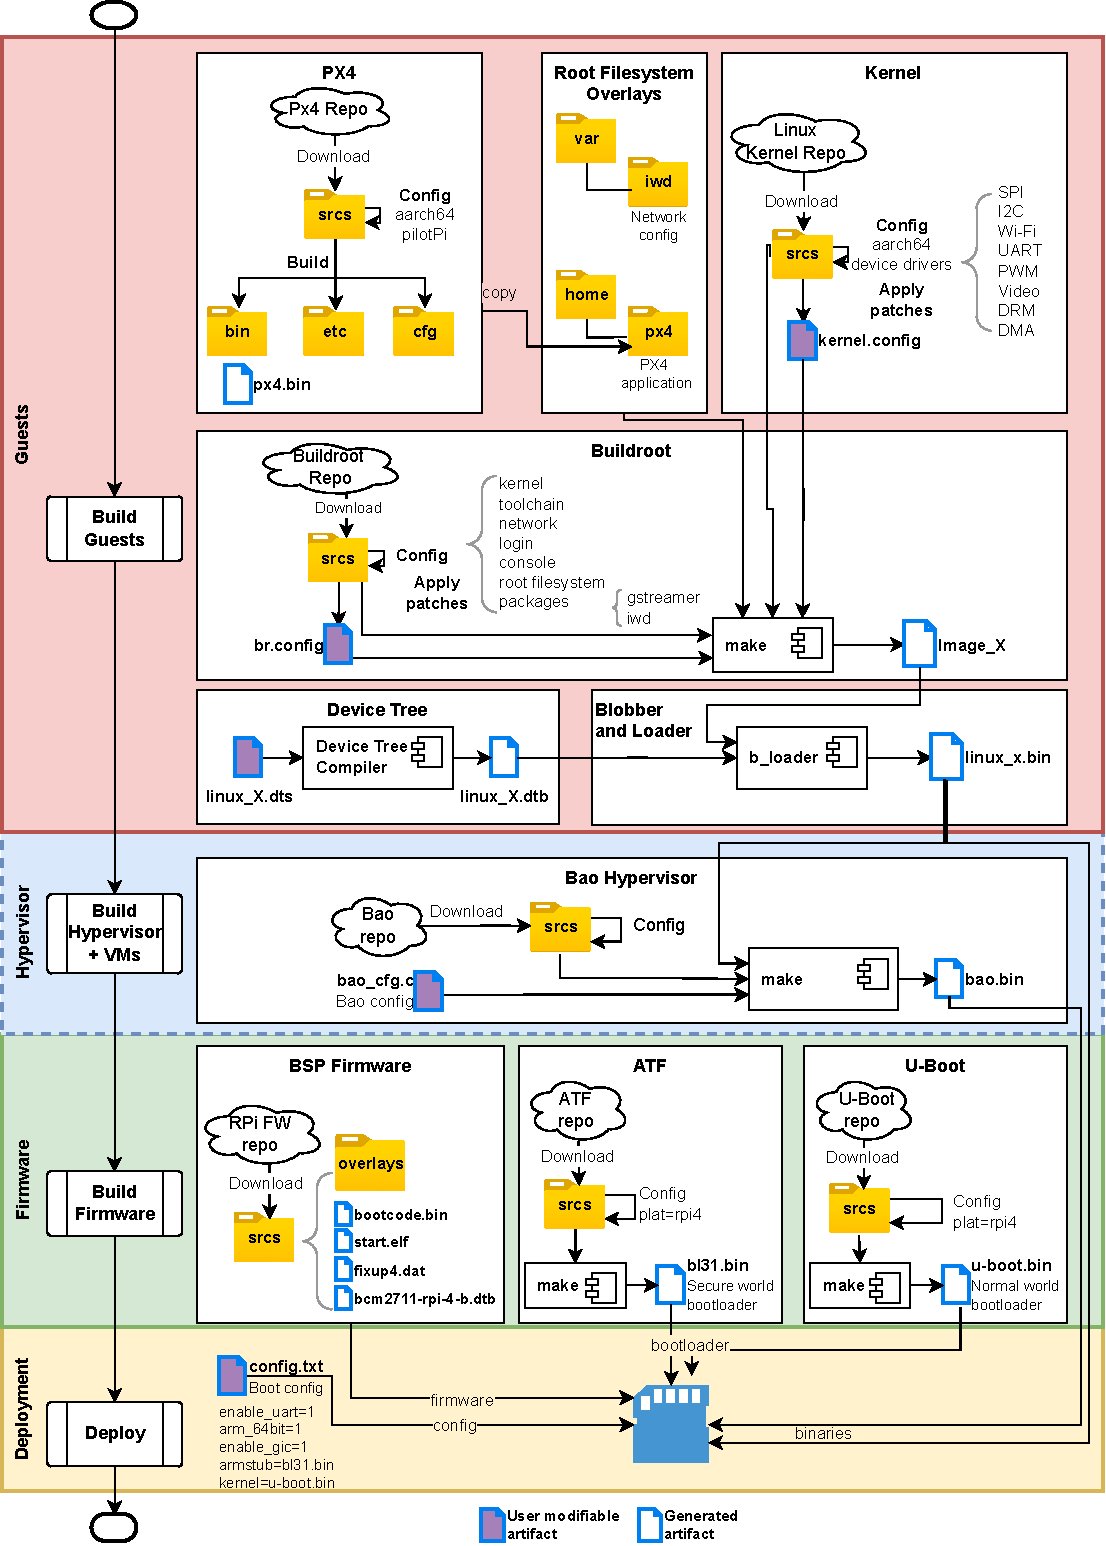
\includegraphics[width=1.0\textwidth]{./img/pdf/uav-main-Implem-Workflow} 
  \caption{Implementation workflow}%
  \label{fig:uav-main-Implem-Workflow}
\end{figure}

% \subsection{Guest Construction}
First we build the guests and its components. In the \gls{uspfs} system, a
single binary wraps the PX4 and video surveillance functionality, while in the
\gls{sspfs} the PX4 and video surveillance guests execute concurrently and in
isolation.
The PX4 application build process targets the \lstinline{PilotPi} board's
\lstinline{aarch64} architecture, generating PX4 binaries and the associated
configuration files to be used at runtime. These files are then copied to Buildroot's root
filesystem directories, alongside with the network configurations, to ensure its deployment within the guest.

The Linux kernel configuration adds support for essential device drivers
(\gls{spi}, \gls{i2c}, Wi-Fi, video, etc.), which is used to deploy the PX4
application with network, login, console, and package support (e.g.,
\lstinline{gstreamer} for video, \lstinline{iwd} for wireless). Next, we use
Buildroot to compile a Linux image
\lstinline{Image_X} (where X denotes guest numbering). We configure the device tree source
\lstinline{linux_X.dts} to match guest-specific hardware and compile to a
\gls{dtb} \lstinline{linux_X.dtb}. Then, the \lstinline{b_loader}
component combines \gls{dtb} and Linux image into a deployable executable with
minimal dependencies. This stage is concluded for the \gls{uspfs} system after
the generation a single binary. On the other hand, the \gls{sspfs} requires this
process to be repeated for each guest, producing two binaries later merged by
Bao. Additionally, we configure \gls{sspfs} system to run atop of the Bao
hypervisor. The \lstinline{bao_cfg.c}) specifies guest build paths, entry
points, \glspl{cpu} allocation, memory regions, and device memory/interrupt
mappings. We then build the Bao hypervisor, which generates a consolidated blob
(\lstinline{bao.bin}) encapsulating both guests atop the hypervisor.
 
% \subsection{Firmware Compilation}
Next, we build the firmware required to boot the platform. We begin by
downloading the Raspberry Pi 4 \gls{bsp}. Then, we configure and build the
\gls{atf} (\lstinline{bl31.bin}), required by Bao, followed by the normal world
bootloader (\lstinline{u-boot.bin}). U-boot is responsible for loading the
target binary, namely \lstinline{linux_x.bin} in the \gls{uspfs} case or
\lstinline{bao.bin} in the \gls{sspfs} one.
% \subsection{Deployment}
Lastly, in the deployment stage, we store the boot artifacts in the \gls{sd}
card: Raspberry Pi firmware, secondary bootloaders, target binary
(\lstinline{linux_x.bin} or \lstinline{bao.bin}), and configuration file
(\lstinline{config.txt}).

However, to successfully deploy the target binary into the platform, we need to
analyze carefully the \gls{uavic} boot flow. Fig.~\ref{fig:uav-main-rpi4-boot}
illustrates the \gls{sd} card layout for the deployment and the \gls{uavic} boot flow. The first stage bootloader
(\lstinline{bootcode.bin}) initializes hardware, loads the firmware from the
\gls{sd} card into \gls{ram}, and parses the boot parameters from
\lstinline{config.txt}.
%
Next, the \lstinline{start4.elf} firmware processes \lstinline{config.txt}, enabling \gls{uart} and \gls{gic} subsystems and hands off execution to the
secondary bootloaders \lstinline{bl31.bin}, which initializes secure services.
%
Then, \lstinline{u-boot.bin} initializes peripherals (including console) using
the firmware's \gls{dtb} and environment variables.
Now, we are able to load the target binary and execute it. We will focus on
\gls{sspfs} case, since it is more generic.
When \lstinline{bao.bin} is executed it starts by: (1) initializing the
\gls{cpu}, the memory, and the system console; (2) configuring the interrupt
manager; (3) initializing the mailbox supervisor; (4) starting the \gls{vm}
manager.
%
After initialization, each \gls{vm}: (1) boots its Linux guest using the
embedded \gls{dtb}; (2) initializes guest-specific hardware; (3) mounts the root
filesystem; (4) and launches the \lstinline{init} process. This results in
isolated guest execution under Bao hypervisor supervision.

\begin{figure}[!hbt]
  \centering
  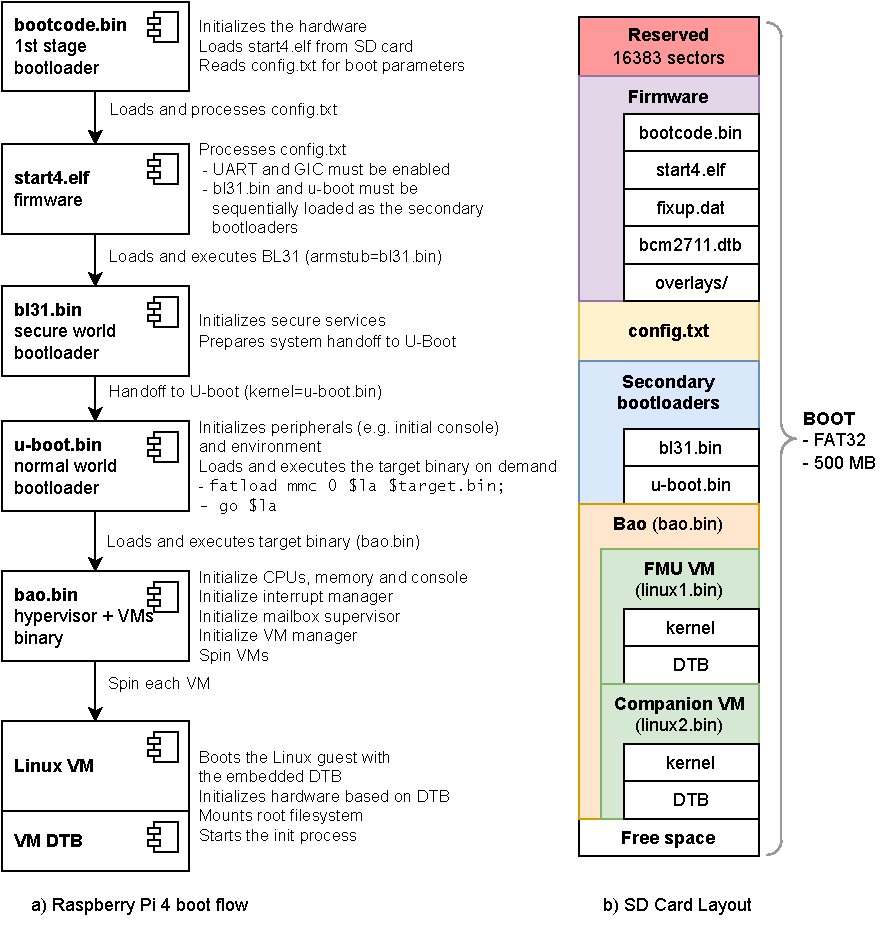
\includegraphics[width=0.9\textwidth]{./img/pdf/uav-main-rpi4-boot} 
  \caption{UAVIC boot: a) platform boot flow; b) SD card layout}%
  \label{fig:uav-main-rpi4-boot}
\end{figure}

\section{Base system}
\label{sec:base-system}
The base system represents the common set of hardware and software components
required for the implementation of the \gls{uspfs} and the \gls{sspfs}
solutions. It comprises the \gls{uav}'s assembly and configuration, and the
testing and validation of the PX4 and video surveillance stacks in isolation.

\subsection{UAV assembly}
\label{sec:uav-assembly}
The initial implementation phase involves \gls{uav} assembly and configuration
using the \gls{gcs} ground station software. Fig.~\ref{fig:uav-assembly}
shows the assembled \gls{uav} based on the HoverGames kit alongside the
QGroundControl \gls{gcs} interface.
%
We started the assembly using with the S500 frame (3) as the structural
foundation, and then incorporating the landing gear, the arms, and the electronics support plates. The NEO-M8N
\gls{gps} module (1) was selected for its cost-effectiveness and performance in
urban environments~\cite{gps-neom8n-product}. Four brushless \gls{dc} motors (2)
were mounted at the arm extremities, controlled by optocoupled 40 Ampere \glspl{esc}.

Power is supplied by a 3S \gls{lipo} battery (12) with 5000 mAh capacity and
XT-60 connector (4)~\cite{lipo-3s-uav}, providing approximately 30 minutes of
full-throttle operation. The \gls{uavic} platform (7) combines the Raspberry Pi
4 with the PilotPi shield. Telemetry radio links (5)(6) enable communication
between the \gls{uav} and QGroundControl \gls{gcs} (11). To facilitate
the early stages of development, we installed and configured a
debug \gls{uart} port (8), which was excluded from the final implementation. The
Wi-Fi dongle (9) and camera (10), required for video surveillance, were
connected via \gls{usb} to the \gls{uavic}.
%
Before starting to configure the \gls{uav}, we must deploy PX4 to the
\gls{uavic}. Only after this, we can communicate with QGroundControl via telemetry radio or Wi-Fi for parameter setup.

\begin{figure}[!hbt]
  \centering
  \includegraphics[width=0.8\textwidth]{./img/png/uav-assembly-annot-final} 
  \caption[UAV assembly and configuration]{UAV assembly and configuration: UAV
    (left); Ground Station running QGroundControl (right)}%
  \label{fig:uav-assembly}
\end{figure}

\subsection{PX4}
\label{sec:px4}
After validating the assembly, we deployed PX4 on top of a general-purpose Linux
\gls{os} on the \gls{uavic} platform. The PX4 build process is detailed in
\lstinline{src/buildPilot.sh} (see~\cite{thesis-sw-github}) and requires a
Python virtual environment to handle dependencies. We downloaded the autopilot
source download, supporting the integration of the NuttX applications (via
submodules); Then we configured and compiled PX4 for the PilotPi board. Lastly,
we deployed PX4 directly to the \gls{uavic} using a Wi-Fi connection.
%
The NuttX \gls{rtos} can be configured using the \lstinline{kconfig} system,
similarly to Linux. Listing~\ref{lst:cfg-pilotpi} presents a configuration
excerpt (see \lstinline{configs/px4/px4.config} for a full version~\cite{thesis-sw-github}) that selects the platform/architecture, sets up the toolchain setup, and
enables all modules and device drivers required.

\begin{longlisting}
\centering
\inputminted[]{kconfig}{./listing/px4.config}
\caption{PX4 configuration file (excerpt)}
\label{lst:cfg-pilotpi}
\end{longlisting}

PX4 runs a boot script, named \lstinline{pilotpi_mc.config} (see
\lstinline{configs/px4/pilotpi_mc.config} for the full
version~\cite{thesis-sw-github}) at startup to configure the \gls{uav} and
enable important services, namely:
\begin{enumerate}[noitemsep,topsep=0pt]
\item Import saved \gls{uav} parameters
\item Configure the vehicle type and airframe
\item Setup the camera to be triggered via Mavlink
\item Initalize the geofence, \gls{cpu} monitoring, and battery status services
\item Initializate sensors and actuators
\item Launch the \gls{rc} communication manager
\item Start the main \gls{fmu} state machine
\item Initialize multicopter-specific tasks: navigation, position/attitude
  control, logging, etc.
\item Enable Mavlink communications, i.e., the telemetry radio and Wi-Fi links
\item Signal to the \gls{gcs} that the boot is complete, delegating further
  configuration to the user
\end{enumerate}

Fig.~\ref{fig:uav-cfg-px4-boot} demonstrates PX4 is successfully
initialized. The sensors and actuators are correctly started and we have
available an active Wi-Fi link (\lstinline{partner IP: 192.168.1.37}) to communicate with the \gls{gcs} via Mavlink.
  
\begin{figure}[!hbt]
  \centering
  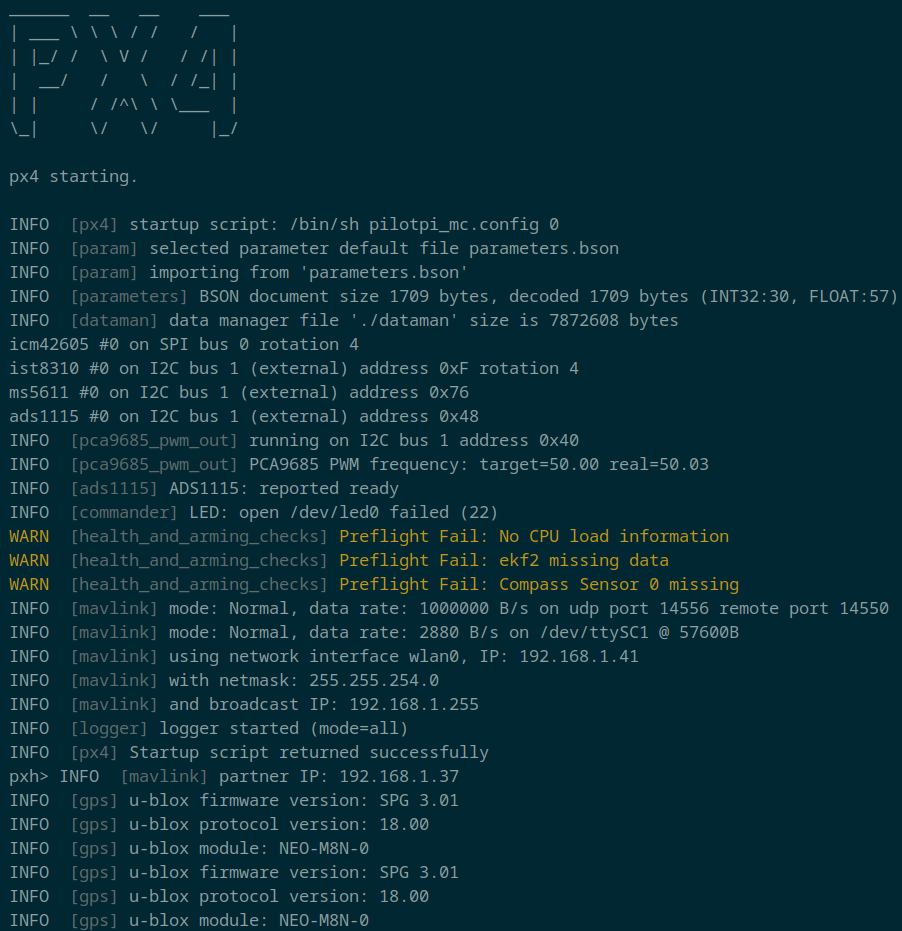
\includegraphics[width=0.6\textwidth]{./img/png/px4-boot} 
  \caption{UAV configuration: PX4 boot}
  \label{fig:uav-cfg-px4-boot}
\end{figure}

\subsection{UAV configuration}
\label{sec:uav-configuration}
After pairing the \gls{uav} to the \gls{gcs}, we can start to configure
it. First, we need to define the UAV's airframe, which in this case is the
quadrotor NXP HoverGames variant (see Fig.~\ref{fig:uav-cfg-airframe}).
Then, we calibrated the compass, gyroscope, and accelerometer sensors by
manipulating the \gls{uav} through the prescribed motions in the \gls{gcs},
gyroscope, and accelerometer (Fig.~\ref{fig:uav-cfg-sensors}).
Next, we configured the power source parameters and battery cells to enable
correct power measurements and calibrated \gls{esc} \gls{pwm} minimum/maximum
values to prevent output saturation.
Lastly, we calibrated the motors, specifying
the motor count and geometry (position/direction) and assigning motors to output
channels. Finally, we tested the motors operation to ensure they spin with the
correct direction and velocity.
Fig.~\ref{fig:uav-cfg-summary} presents the configuration summary, showcasing
that the \gls{uav} is correctly set up. The established parameter database can
then be replicated across multiple PX4 instances to bootstrap identical \glspl{uav}.

\begin{figure}[!hbt]
  \centering
  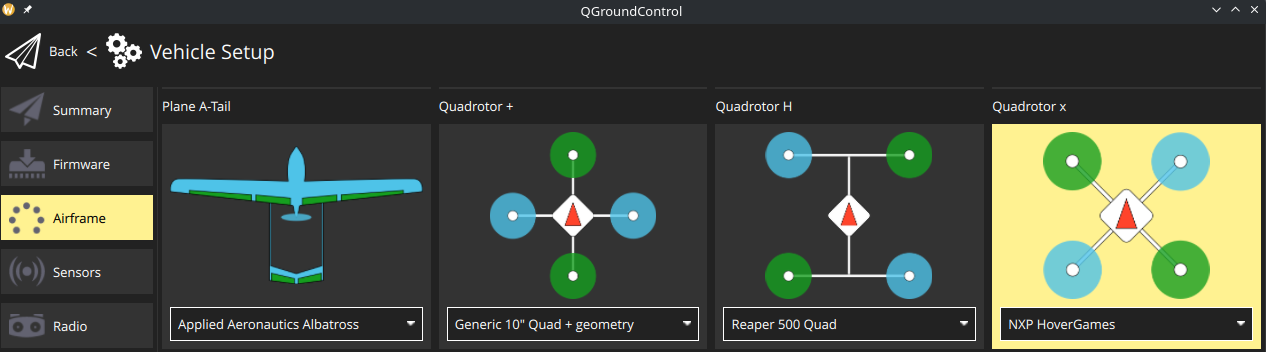
\includegraphics[width=0.9\textwidth]{./img/png/qgc-airframe} 
  \caption{UAV configuration: airframe}
  \label{fig:uav-cfg-airframe}
\end{figure}

\begin{figure}[!hbt]
  \centering
  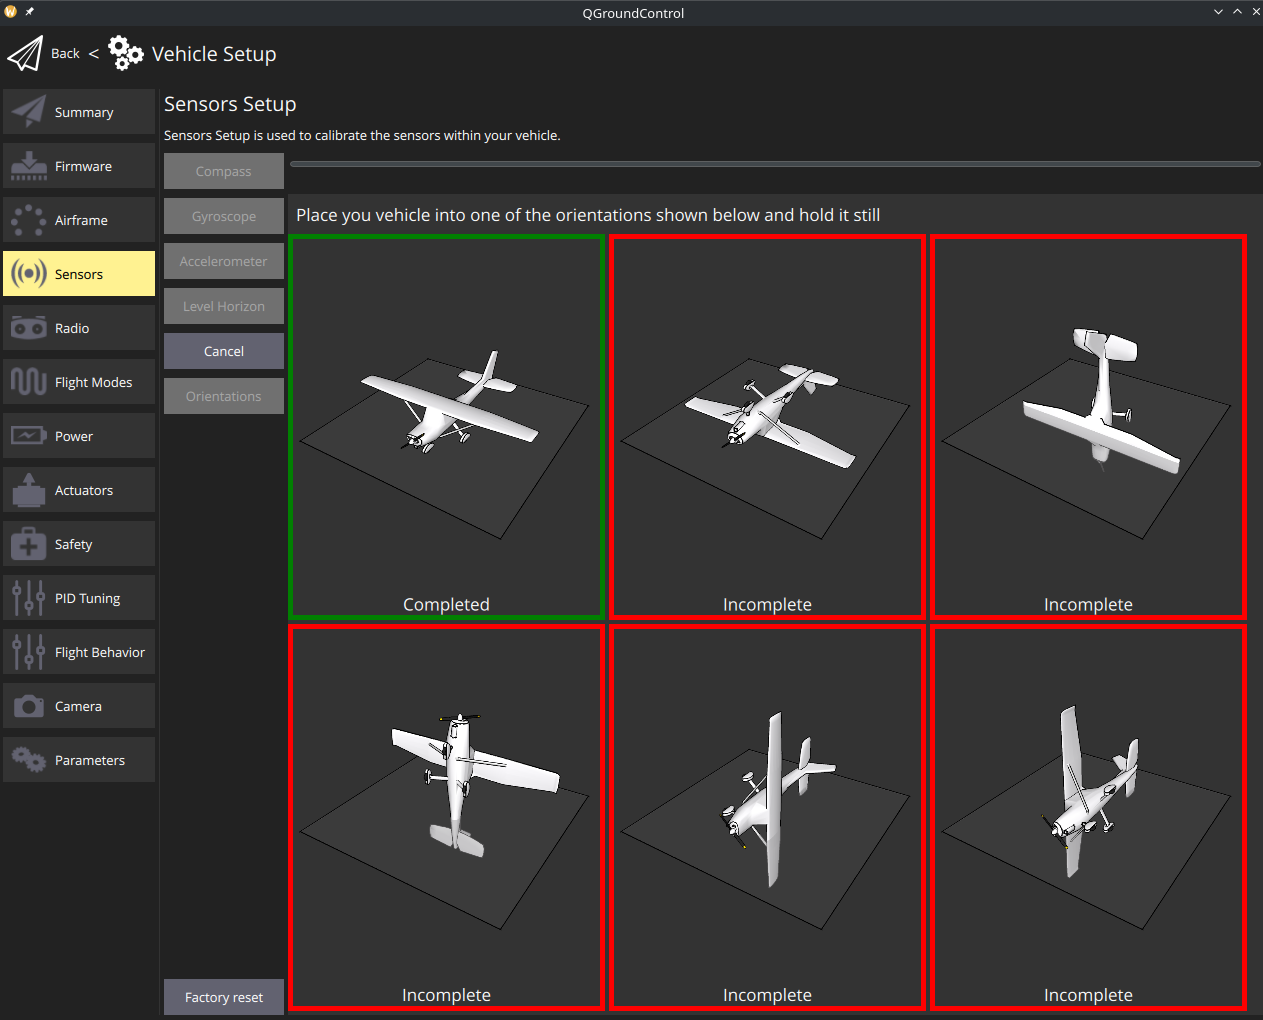
\includegraphics[width=0.9\textwidth]{./img/png/qgc-sensors} 
  \caption{UAV configuration: sensors' calibration}
  \label{fig:uav-cfg-sensors}
\end{figure}

% \begin{figure}[!hbt]
%   \centering
%   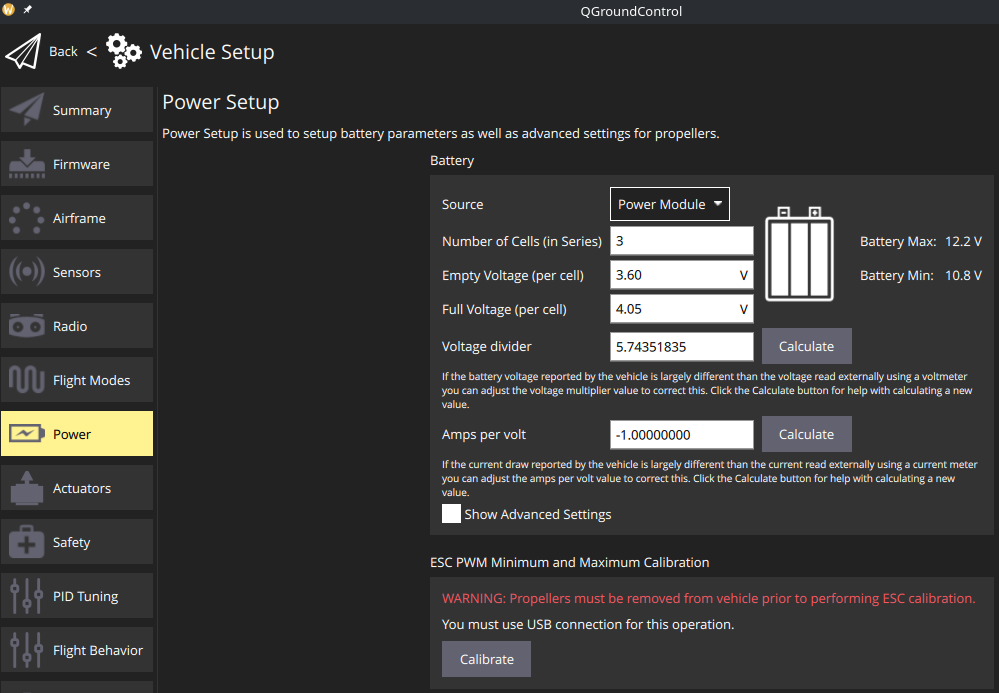
\includegraphics[width=0.8\textwidth]{./img/png/qgc-power} 
%   \caption{UAV configuration: power management}
%   \label{fig:uav-cfg-power}
% \end{figure}

% \begin{figure}[!hbt]
%   \centering
%   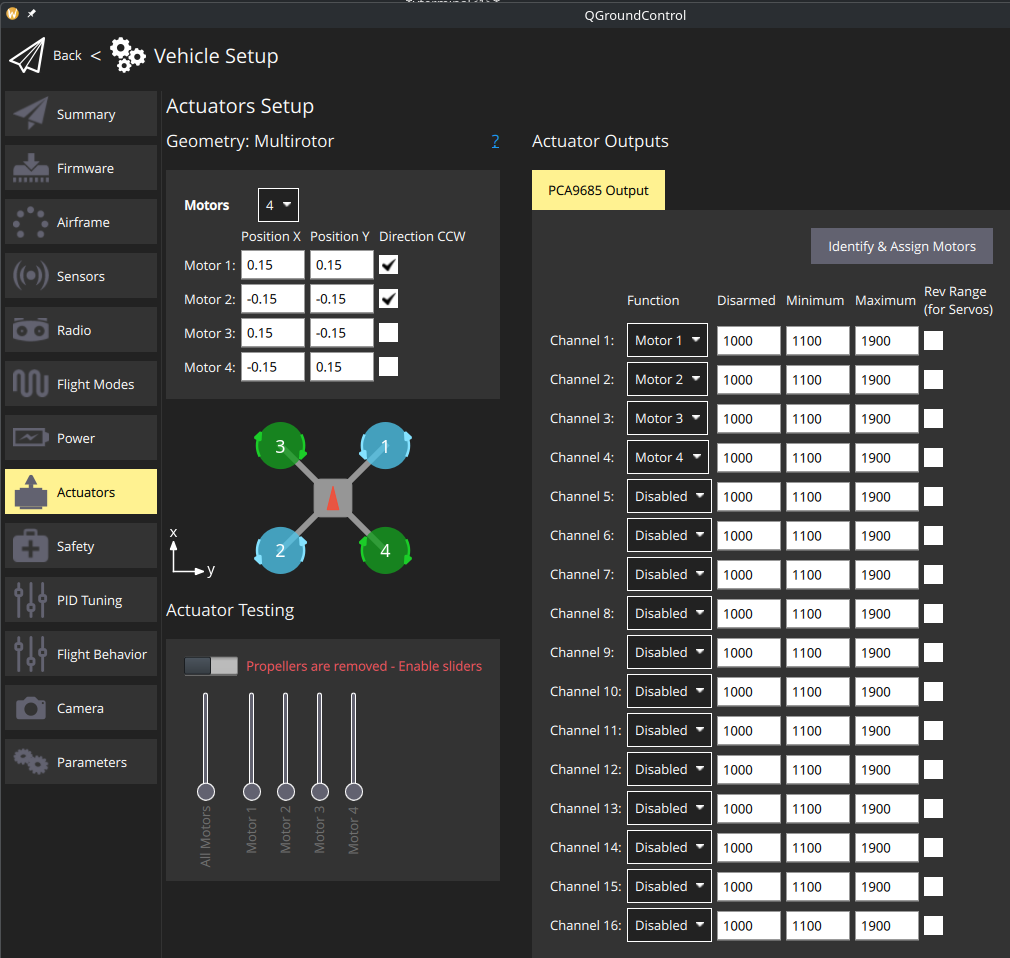
\includegraphics[width=0.75\textwidth]{./img/png/qgc-actuators} 
%   \caption{UAV configuration: actuators}
%   \label{fig:uav-cfg-actuators}
% \end{figure}

\begin{figure}[!hbt]
  \centering
  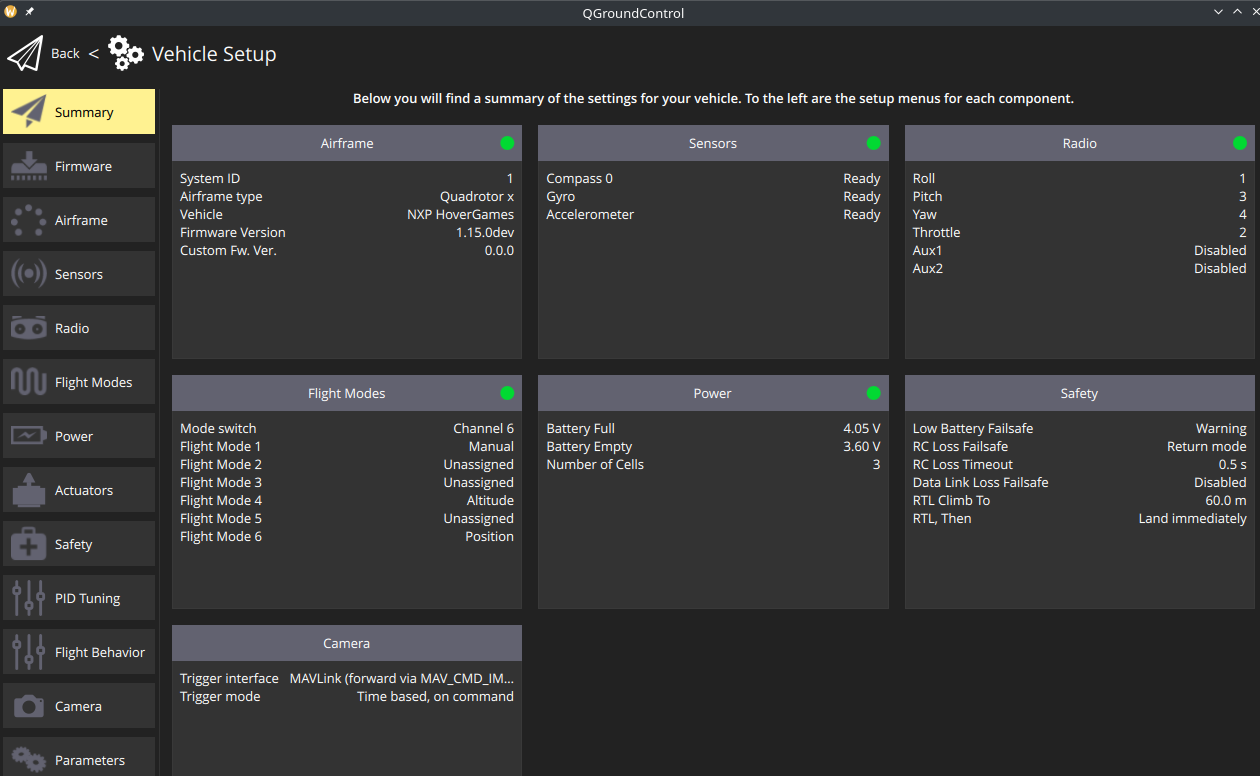
\includegraphics[width=0.92\textwidth]{./img/png/qgc-summary} 
  \caption{UAV configuration: summary}
  \label{fig:uav-cfg-summary}
\end{figure}

\subsection{Video surveillance}
\label{sec:video-surveillance}
The video surveillance pipeline,  illustrated in
Fig.~\ref{fig:uav-design-unsup}, was implemented and validated using the
\lstinline{gstreamer} multimedia framework. This open-source framework has a
modular architecture supporting several video codecs and network streaming
capabilities, enabling rapid iteration and simplified testing.
%
The \textbf{sender} component, executing on the \gls{uav}, performs frame
capture at designated resolution/framerate in MJPEG format, followed by frame
decoding, H.264 encoding, and \gls{rtsp} packaging for \gls{udp} transmission.
Listing~\ref{lst:gstreamer-sender} details the sender pipeline test script,
specifying the USB camera device at 640×480 resolution and 30 \gls{fps}, along
with host \gls{ip}/port configuration ensuring exclusive \gls{gcs} reception.

\begin{longlisting}
\centering
\inputminted[]{bash}{./listing/gstreamerSender.sh}
\caption{Video surveillance sender script}
\label{lst:gstreamer-sender}
\end{longlisting}

Conversely, the \textbf{receiver} component on the \gls{gcs} connects to the designated \gls{udp} port, decodes and unpacks the \gls{rtsp} stream, converts to display format, and renders video output.
Listing~\ref{lst:gstreamer-receiver} shows the receiver test script, configuring the matching \gls{udp} port, H.264 decoding, and \lstinline{autovideosink} for display.

\begin{longlisting}
\centering
\inputminted[]{bash}{./listing/gstreamerReceiver.sh}
\caption{Video surveillance receiver script}
\label{lst:gstreamer-receiver}
\end{longlisting}

We then validated the whole pipeline (Fig.~\ref{fig:px4-qgc-cam}) by executing concurrently: (1) the PX4
flight stack (Fig.~\ref{fig:px4-qgc-cam-2}) and the video surveillance sender on
top of a general purpose Linux \gls{os}
within the \gls{uavic} (Fig.~\ref{fig:px4-qgc-cam-3}, top); (2) the video receiver
and QGroundControl on the \gls{gcs} (Fig.~\ref{fig:px4-qgc-cam-3}, bottom).
Fig.~\ref{fig:px4-qgc-cam-1} shows that \gls{uav} telemetry is displayed in
QGroundControl alongside the video stream, validating the video surveillance pipeline.

\begin{figure}[htb!]
  \centering
  %
  \begin{subfigure}[t]{.48\textwidth}
    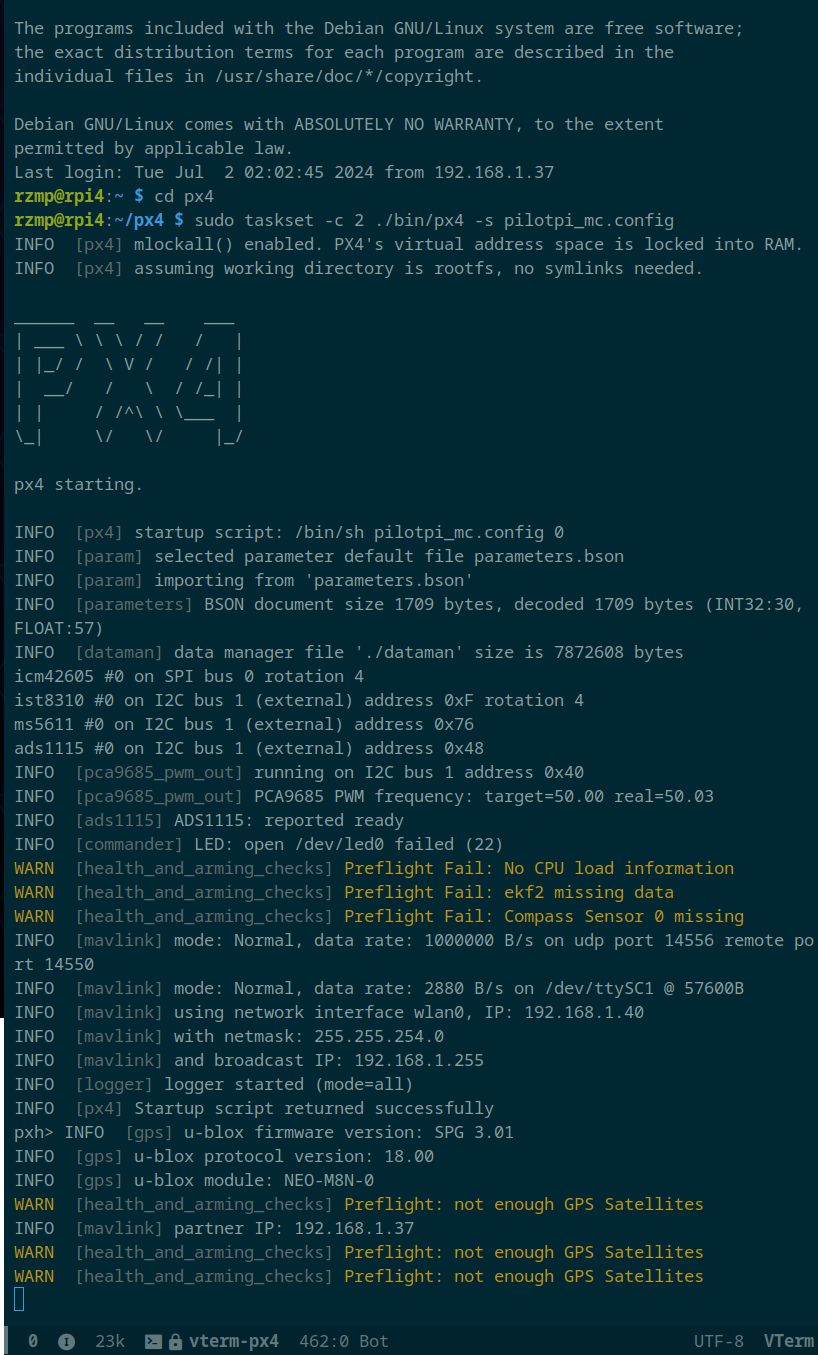
\includegraphics[width=0.89\textwidth]{./img/png/px4-qgc-cam-2}
  \caption{PX4 boot}%
  \label{fig:px4-qgc-cam-2}
  \end{subfigure}
%
  \begin{subfigure}[t]{.48\textwidth}
    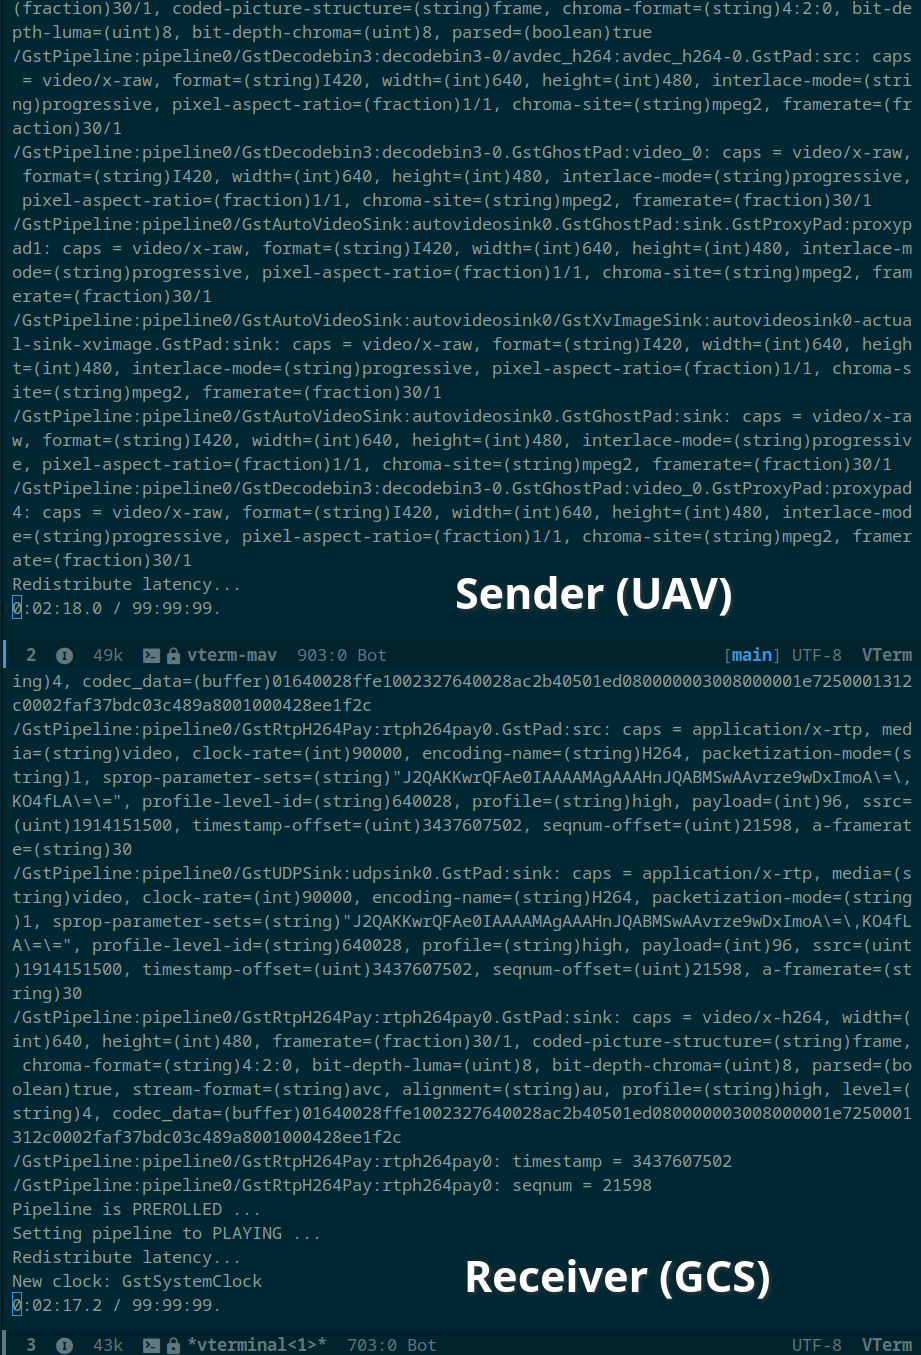
\includegraphics[width=1.0\textwidth]{./img/png/px4-qgc-cam-3}
  \caption{Video pipeline: sender (UAV); receiver (GCS)}%
  \label{fig:px4-qgc-cam-3}
  \end{subfigure}
%
  \begin{subfigure}[t]{.48\textwidth}
    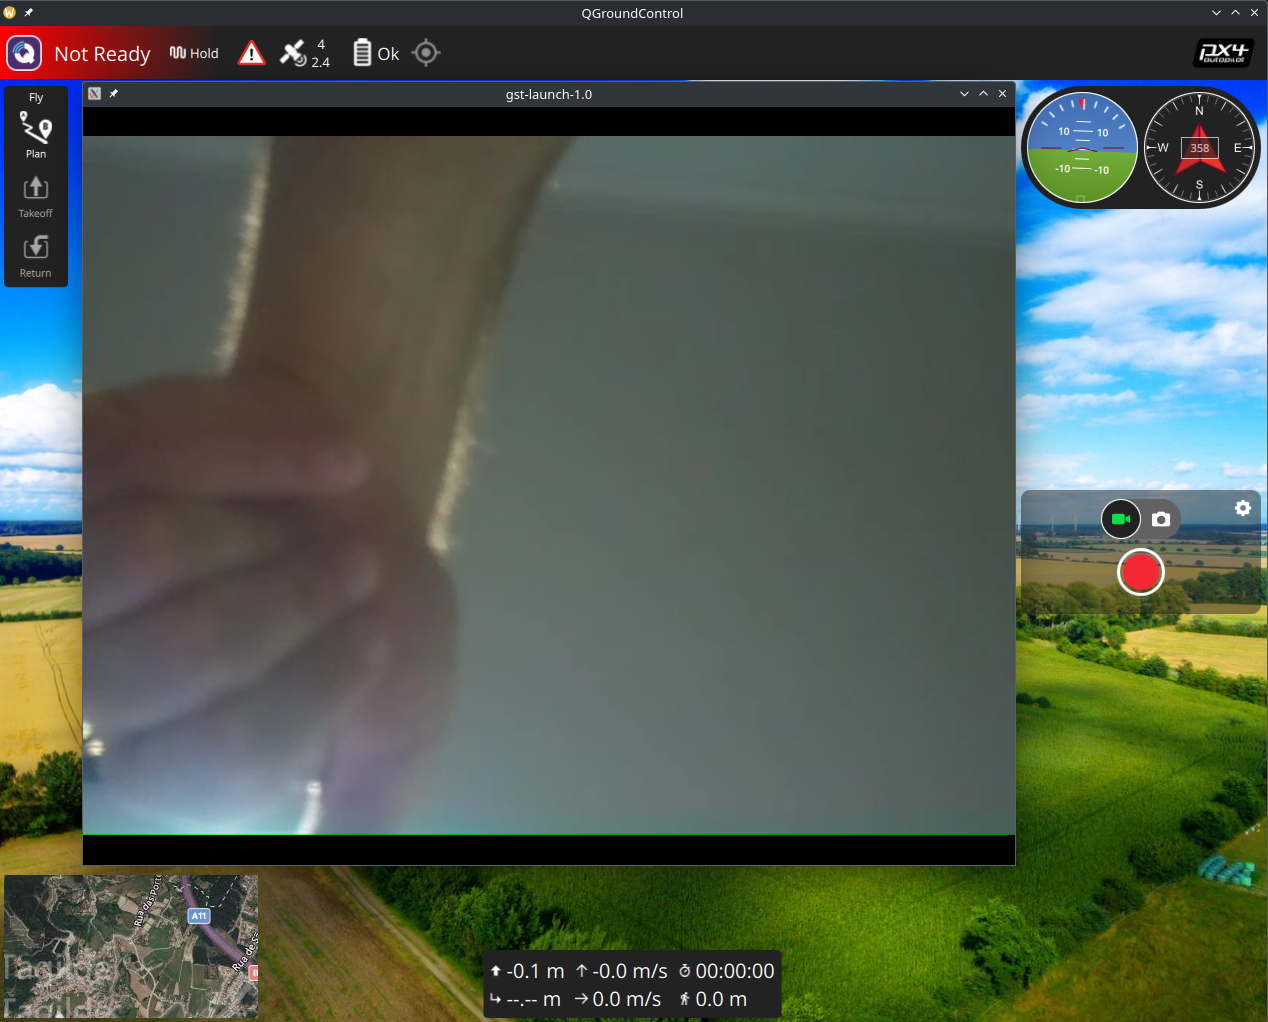
\includegraphics[width=1.0\textwidth]{./img/png/px4-qgc-cam-1}
  \caption{QGroundControl and video surveillance receiver}%
  \label{fig:px4-qgc-cam-1}
  \end{subfigure}
  % 
  \caption{Video surveillance pipeline validation}%
  \label{fig:px4-qgc-cam}
\end{figure}

\section{USPFS}
\label{sec:uspfs-implem}
The \gls{uspfs} solution consolidates PX4 and video surveillance functionality
within a custom embedded Linux-based \gls{os} on the \gls{uavic}.
We started by configuring a stable kernel for the Raspberry Pi (version 6.6)  to
support both software stacks and the associated device drivers and modules.
The detailed kernel configuration is available in
\lstinline{configs/uspfs/kernel-uspfs.config} (see~\cite{thesis-sw-github}). PX4
requires the following device drivers: \gls{spi}/\gls{i2c} for sensors and
actuators; \gls{pwm} for motors; and PL011 for \gls{rc} and \gls{uart}. On the other
hand, the video surveillance requires the video device drivers and the \lstinline{MT7921U} module for Mediatek Wi-Fi dongle support.

Then, we configured Buildroot (see \lstinline{configs/uspfs/br-uspfs.config}) to:
(1) integrate our custom kernel; (2) add the root filesystem overlay containing
the PX4 binaries; (3) setup the boot debug console to UART5
(\lstinline{ttyAMA5}); (4) add the \lstinline{GStreamer} package for video
support; (5) add the Mediatek firmware for the \gls{usb} Wi-Fi dongle support.
After this, we were able to compile our custom Linux \gls{os} image (\lstinline{Image_1}).   
Next, we customized a device tree that incorporates all necessary hardware
(see Fig.~\ref{fig:hw-map-1}), and combined it with the Linux OS image to
generate an executable \lstinline{linux_1.bin} blob.

Then, we downloaded the Raspberry Pi 4 \gls{bsp} and patched the secondary
bootloader (\lstinline{bl31.bin}) to support UART5 (\lstinline{ttyAMA5}) debug
console instead of the default UART0. The \lstinline{configs/atf/atf-patch.mk}
file~\cite{thesis-sw-github} shows the inline replacement of \lstinline{serial0}
with \lstinline{serial5} and the modification of the \gls{uart} offset. Next, we
customized U-boot (\lstinline{configs/uboot/uboot.mk} and \lstinline{configs/uboot/uboot.env}~\cite{thesis-sw-github})
to enable automatic binary loading at a designated address following the \lstinline{bl31.bin} execution.

Finally, we wrote the boot artifacts into the SD card: the custom image
(\lstinline{linux_1.bin}), Raspberry Pi firmware, secondary bootloaders, and
\lstinline{config.txt}. The \lstinline{config.txt} (see
\lstinline{configs/uspfs/config.txt}~\cite{thesis-sw-github}) configures the
\gls{gic} subsystem for early interrupts, specifies the secondary bootloader and
kernel to boot the platform, and configures UART5 as the system console.
%
Lastly, we validated the whole process by inserting the SD card into the
\gls{uavic} and monitoring boot process via terminal emulator (\lstinline{screen /dev/ttyUSB0 115200}).
The boot log, available at
\lstinline{logs/boot-uspfs.txt}~\cite{thesis-sw-github}, confirms the Linux
kernel/Buildroot toolchain versions and UART5 console initialization.
We then ran the same test procedures from Sections~\ref{sec:px4}
and~\ref{sec:video-surveillance}, and verified the correct execution of both PX4 and video surveillance applications in the \gls{uspfs} environment.

\section{SSPFS}
\label{sec:sspfs-implem}
For the \gls{sspfs} system we need to build two isolated Linux \glspl{os}
(guests) running atop the Bao hypervisor: one for PX4 and another for video
surveillance.
The guest generation process is very similar to the \gls{uspfs} process one. For
each guest:
(1) we select the kernel, device drivers, packages and compiled them into a
separate Linux \gls{os} image (\lstinline{Image_X});
(2) we customize the Linux device tree;
(3) we build an executable blob from the \gls{os} image and the device tree,
namely \lstinline{linux_1.bin} (PX4) and \lstinline{linux_2.bin} (video
surveillance).

%\subsection{Hypervisor and VM Construction}
We forked the Bao hypervisor into another repository~\cite{baoRepo-mine} to comply with
\gls{sspfs}-specific requirements, namely modifying the default console address,
clock frequency and offset from UART0 to UART5 in the Raspberry Pi 4 platform.
Firstly, we modified the console base address in the platform description file
(see \lstinline{src/rpi4_desc.c}~\cite{thesis-sw-github}) to
\lstinline{0xfe201000} (4KB-aligned). Then, in the platform header file \lstinline{src/platform.h}~\cite{thesis-sw-github}, we set UART5's clock frequency to 48
MHz and its address offset to \lstinline{0xa00}, yielding the UART5 address
(\lstinline{0xfe201a00}).
We then allocated the platform resources to each guest within Bao (see
\lstinline{configs/sspfs/bao_sspfs_cfg.c}~\cite{thesis-sw-github}). PX4 \gls{vm}
has a primary memory region of 144 MB and a secondary one of 3 GB. The memory
separation happens because the \gls{dma} transactions are mapped in the first 1
GB of \gls{ram}. We assign one core to this \gls{vm} and 9 devices
(Fig.~\ref{fig:hw-map-2}). For the video \gls{vm} we reserve 624 MB of \gls{ram}
to run the memory-intensive video pipeline and an optional 2 GB memory
region. We assign the remaning 3 cores to this VM and 4 devices
(Fig.~\ref{fig:hw-map-3}).
Shared devices, such as the architectural timer and mailbox, require special
handling. The first is managed automatically by Bao, while we must implement the
second to enable access to \gls{pcie} devices in the video \gls{vm}.

\subsection{Mailbox Supervisor}
The mailbox supervision mechanism (Fig.~\ref{fig:design-mailbox}) implementation
integrates two critical components: (1) the addition of a mailbox manager
addition to Bao; (2) a patch to the Raspberry Pi mailbox's firmware driver
within the Linux kernel.
Listing~\ref{lst:bao-mailbox-manager} shows the mailbox manager implementation.
We defined a specific interrupt identifier to signal the mailbox's hypercall
and arguments to identify the start and end of a mailbox transaction. The
function \lstinline{plat_rpi_init} is called when the platform is initialized
(see \lstinline{src/init.c}~\cite{thesis-sw-github}) and before \gls{vm}
startup, associating the mailbox's interrupt to the
\lstinline{rpi_mailbox_irq_handler}. This function is then called when the
mailbox transaction is detected within Bao and injects into the current virtual
\gls{cpu} the interrupt \lstinline{id} and prevents Bao from handling this
interrupt request as a normal one. This triggers an hypercall (defined in
Listing~\ref{lst:bao-hypercall}), which in turn calls back the \lstinline{rpi_mailbox_hypercall}
function. This function then grants the current \lstinline{vCPU} exclusive access to the mailbox to handle the transaction, enabling the interrupts at the
start and disabling them in the end.

\begin{longlisting}
\centering
\inputminted[]{c}{./listing/rpi_firmware.c}
\caption[SSPFS: mailbox manager added to Bao]{SSPFS: Mailbox manager added to
  Bao (see \lstinline{src/rpi_firmware.c}~\cite{thesis-sw-github})}  
\label{lst:bao-mailbox-manager}
\end{longlisting}

\begin{longlisting}
\centering
\inputminted[]{c}{./listing/hypercall.c}
\caption[SSPFS: Bao hypercall manager]{SSPFS: Bao hypercall manager (see \lstinline{src/rpi_firmware.c}~\cite{thesis-sw-github})}
\label{lst:bao-hypercall}
\end{longlisting}

The hypercall manager
(Listing~\ref{lst:bao-hypercall}) acts as a common interface that the Linux
device driver must adhere to when triggering the hypercall: its
\lstinline{id} (\lstinline{HC_RPI_FIRMWARE}) and the transaction's start and end
arguments. The hypercall manager reinjects these arguments into its callback,
ensuring consistent behavior.
%
Listing~\ref{lst:linux-rpi-fw}) shows the patch done in the Linux mailbox
driver. We define the same hypercall \lstinline{id} and arguments. After locking
the access to the mailbox, we explicitly trigger a hypercall through the
\lstinline{hvc} assembly instruction with the start argument. This hypercall
must happen before the mailbox handling the actual transaction. When the
transaction is finished we trigger another hypercall, but now with the end
argument, and unlock the mailbox, finalizing the transaction.

\begin{longlisting}
\centering
\inputminted[]{c}{./listing/linux-rpi-fw.c}
\caption[SSPFS: Linux's Raspberry Pi mailbox driver -- patch]{SSPFS: Linux's
  Raspberry Pi mailbox driver -- patch (see \lstinline{src/linux-rpi-fw.c}~\cite{thesis-sw-github})}
\label{lst:linux-rpi-fw}
\end{longlisting}

% \section{Summary}
% \label{sec:summary-implem}
% This chapter detailed the implementation of both \gls{uspfs} and \gls{sspfs} solutions following the established workflow. Base system validation encompassed four critical stages: UAV physical assembly, PX4 compilation and deployment for the target platform, UAV configuration via PX4, and video surveillance pipeline setup with validation.

% The \gls{uspfs} implementation featured deployment of a custom embedded Linux \gls{os} consolidating PX4 and video surveillance stacks, supported by kernel configuration for required drivers/modules. Key modifications included \gls{atf} patching for UART5 console redirection and boot process configuration through U-Boot environment scripts and \lstinline{config.txt}, culminating in successful validation of both software stacks.

% The \gls{sspfs} implementation involved constructing isolated Linux guests for each software stack, with Bao hypervisor customization adding UART5 support. Resource allocation assigned PX4 (1 CPU, 144MB RAM, 9 devices) and Video (3 CPUs, 624MB RAM, 4 devices) their respective resources. Mailbox supervision implementation required coordinated Bao hypervisor modifications and Linux kernel mailbox driver patching. Validation occurred through boot process inspection via UART debug/SSH and functional verification of both software stacks.

% Both solutions were successfully implemented and validated, meeting all functional requirements.

%%% Local Variables:
%%% mode: LaTeX
%%% TeX-master: "../template"
%%% reftex-default-bibliography: ("../Bibliography/mieeic.bib")
%%% ispell-local-dictionary: "american"
%%% End:
